\chapter{Concurrency}\label{ch:concurrency}

The following chapter will focus on the concurrency control of the application. Explaning the problem and the solution that we implemented.

\section{Background}
One of the problems of our project is the concurrency control of the application. Since we have a functionality where multiple users can simultaneously access and modify the same financial data, we need to ensure that the data is consistent and that the users are not overwriting each other's changes. The situations that can happen are:
\begin{itemize}
\item Every operation that modifies the wallet balance (adding a new transaction, updating a transaction, deleting a transaction)
\item Every operation that modifies the limits (creating a new limit, updating a limit, deleting a limit)
\item Every operation that modifies saving goals.
\end{itemize}

All these scenarios share a fundamental challenge on the client-side: users lack visibility into whether another user has already modified the same data before they attempt to submit their changes. To address this issue, the team investigated several potential solutions.

\section{Current Solution}

\begin{figure}[H]
    \centering
    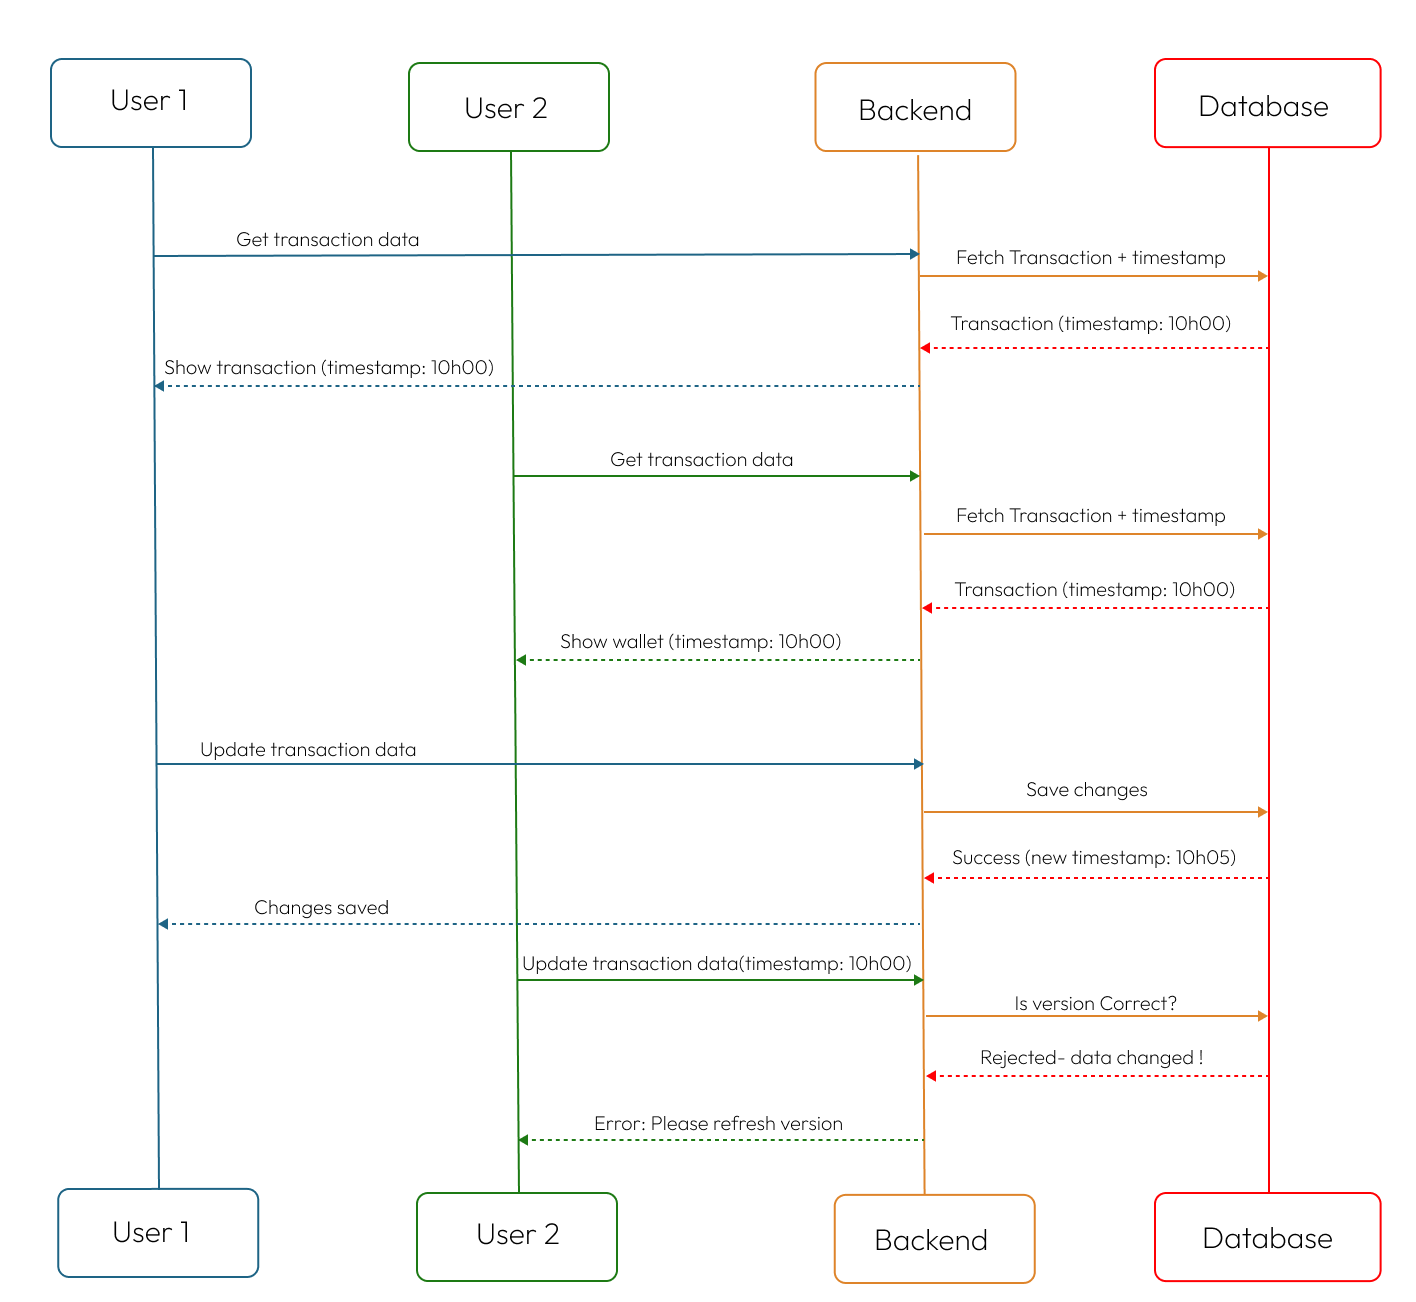
\includegraphics[width=0.9\textwidth]{./img/concurrency.png}
    \caption{Concurrency Control}
    \label{fig:concurrency}
\end{figure}

Our solution draws inspiration from optimistic concurrency control patterns, specifically adapting concepts from a previous university project that implemented similar timestamp-based approaches \textbf{reference to be added}. Rather than using traditional ETag headers with hash values, we implemented a timestamp-based versioning system that operates through the request body. This design provides resource version control similar to ETag protocols while maintaining a clear audit trail of when each update occurred.

The implementation was relatively straightforward since our database schema already included the necessary infrastructure with \textit{updatedAt} fields and similar timestamp structures across all relevant tables. However, we encountered some challenges during the integration process that required careful consideration of the transaction handling and client-server communication flow.

The system operates as follows: all timestamps are saved at the database level upon successful updates, ensuring consistency across the application. When a client component requests data from the server, the response includes both the requested resource and its associated last-modified timestamp.

For update operations, clients must include this timestamp alongside the new data. The server uses this timestamp to verify that no concurrent modifications have occurred since the client retrieved the data. If another user has modified the resource in the meantime, the update will be rejected, preventing data loss and maintaining consistency.

The timestamp verification strategy varies depending on the type of operation being performed. For transaction-related operations (creating, updating, or deleting transactions), the system uses the wallet's updatedAt timestamp rather than the individual transaction's updatedAt timestamp. This approach is necessary because transactions directly affect the wallet's balance, and the system needs to ensure that the user has the most recent version of the wallet before allowing any operation that affects the balance. For operations on saving goals and spending limits, the system uses the item's individual updatedAt timestamp since these entities operate independently and do not directly impact others.

All update operations are executed within database transactions using the default Read Committed isolation level. This transactional approach is essential since Patch requests often modify multiple related tables, and the transaction ensures these changes are treated as an atomic unit of work.

Under the Read Committed isolation level, when an UPDATE statement targets a row that has been modified by another uncommitted transaction, the second transaction waits for the first to either commit or rollback. If the first transaction rolls back, the waiting transaction can proceed. If it commits, the query is re-executed to verify the updated row still meets the search conditions before applying the change.

Figure \ref{fig:concurrency} illustrates the concurrency control flow of this concurrency control mechanism, showing how the timestamp-based approach prevents the race conditions that could otherwise occur in shared wallet scenarios.

\subsection{Limitations}
Since we don't have a real-time notifications system, the following limitations are present:
\begin{itemize}
    \item Users must refresh data and retry operations when conflicts occur.
    \item Client needs to handle refresh logic when operations are rejected.
    \item Frequent rejection messages in busy shared wallets can cause frustration.
    \item Conflict probability increases exponentially with concurrent users.
\end{itemize}
